\begin{figure}
  \centering 
  \begin{subfigure}[b]{0.45\textwidth}
    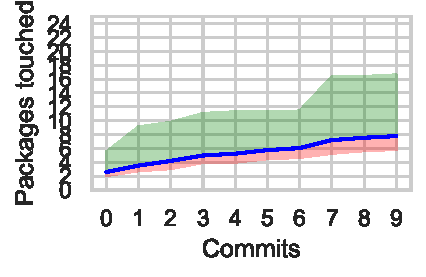
\includegraphics[width=\textwidth]{sections/results/packages/time_series_components_touched.packages.moderate.founder.commits_10.pdf}
    \caption{Moderate founder (n=32, $\mu$=7.75, median=4.0 \& std=6.31)}
    \label{subfig:sections/results/packages/time_series_components_touched_packages_moderate_founder_commits_10_pdf}
  \end{subfigure}
  \begin{subfigure}[b]{0.45\textwidth}
    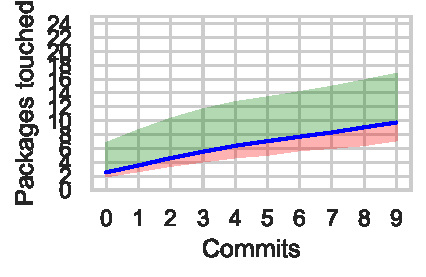
\includegraphics[width=\textwidth]{sections/results/packages/time_series_components_touched.packages.moderate.later.joiner.commits_10.pdf}
    \caption{Moderate later joiner (n=580, $\mu$=9.73, median=5.0 \& std=6.0)}
    \label{subfig:sections/results/packages/time_series_components_touched_packages_moderate_later_joiner_commits_10_pdf}
  \end{subfigure}
\vspace{3mm}
  \begin{subfigure}[b]{0.45\textwidth}
    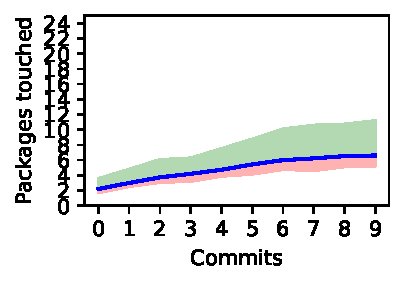
\includegraphics[width=\textwidth]{sections/results/packages/time_series_components_touched.packages.sustained.founder.commits_10.pdf}
    \caption{Sustained founder (n=27, $\mu$=5.96, median=3.0 \& std=4.15)}
    \label{subfig:sections/results/packages/time_series_components_touched_packages_sustained_founder_commits_10_pdf}
  \end{subfigure}
  \begin{subfigure}[b]{0.45\textwidth}
    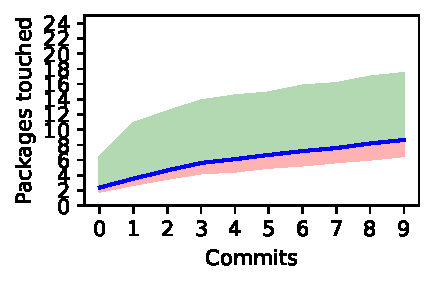
\includegraphics[width=\textwidth]{sections/results/packages/time_series_components_touched.packages.sustained.later.joiner.commits_10.pdf}
    \caption{Sustained later joiner (n=203, $\mu$=8.65, median=4.0 \& std=6.6)}
    \label{subfig:sections/results/packages/time_series_components_touched_packages_sustained_later_joiner_commits_10_pdf}
  \end{subfigure}
\caption[Time Series for packages unit:commits category:4 commits:10]{A time series for the ten (10) commits, excluding transient, with the average mean (blue line), packages touched (y-axis) against the number of commits (x-axis) for four (4) developer categories. Green is the standard deviation above the mean, and pink is the standard deviation below the mean.} 
    \label{fig:codebase_graph_latex_repository_graph_component_time_series_time_series_components_touchedpackages_10_10}
\end{figure}
\clearpage 
\begin{figure}
  \centering 
  \begin{subfigure}[b]{0.45\textwidth}
    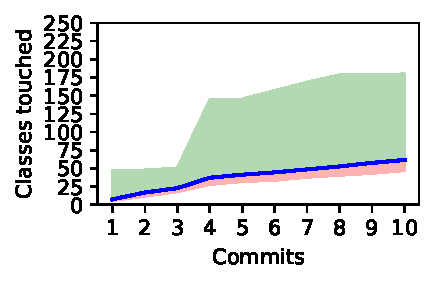
\includegraphics[width=\textwidth]{sections/results/classes/time_series_components_touched.classes.moderate.founder.commits_10.pdf}
    \caption{Moderate founder (n=32, $\mu$=64.88, median=16.0 \& std=77.36)}
    \label{subfig:sections/results/classes/time_series_components_touched_classes_moderate_founder_commits_10_pdf}
  \end{subfigure}
  \begin{subfigure}[b]{0.45\textwidth}
    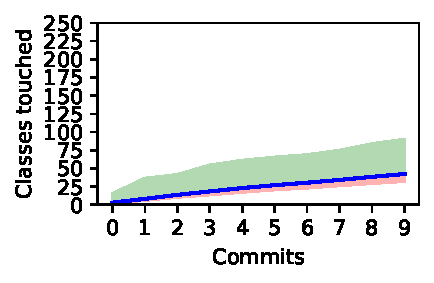
\includegraphics[width=\textwidth]{sections/results/classes/time_series_components_touched.classes.moderate.later.joiner.commits_10.pdf}
    \caption{Moderate later joiner (n=580, $\mu$=41.95, median=14.0 \& std=29.54)}
    \label{subfig:sections/results/classes/time_series_components_touched_classes_moderate_later_joiner_commits_10_pdf}
  \end{subfigure}
\vspace{3mm}
  \begin{subfigure}[b]{0.45\textwidth}
    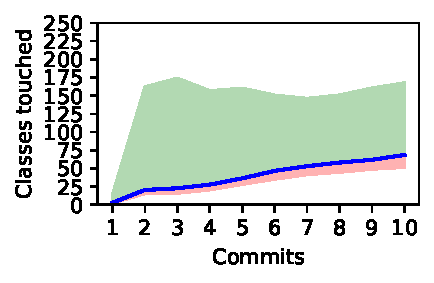
\includegraphics[width=\textwidth]{sections/results/classes/time_series_components_touched.classes.sustained.founder.commits_10.pdf}
    \caption{Sustained founder (n=27, $\mu$=71.37, median=14.0 \& std=78.48)}
    \label{subfig:sections/results/classes/time_series_components_touched_classes_sustained_founder_commits_10_pdf}
  \end{subfigure}
  \begin{subfigure}[b]{0.45\textwidth}
    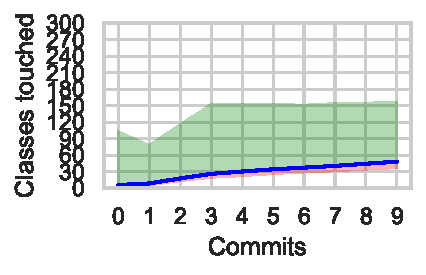
\includegraphics[width=\textwidth]{sections/results/classes/time_series_components_touched.classes.sustained.later.joiner.commits_10.pdf}
    \caption{Sustained later joiner (n=203, $\mu$=47.98, median=13.0 \& std=62.35)}
    \label{subfig:sections/results/classes/time_series_components_touched_classes_sustained_later_joiner_commits_10_pdf}
  \end{subfigure}
\caption[Time Series for classes unit:commits category:4 commits:10]{A time series for the ten (10) commits, excluding transient, with the average mean (blue line), classes touched (y-axis) against the number of commits (x-axis) for four (4) developer categories. Green is the standard deviation above the mean, and pink is the standard deviation below the mean.} 
    \label{fig:codebase_graph_latex_repository_graph_component_time_series_time_series_components_touchedclasses_10_10}
\end{figure}
\clearpage 
\begin{figure}
  \centering 
  \begin{subfigure}[b]{0.45\textwidth}
    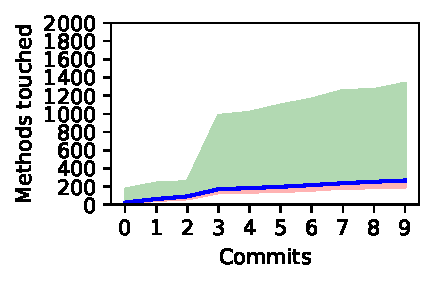
\includegraphics[width=\textwidth]{sections/results/methods/time_series_components_touched.methods.moderate.founder.commits_10.pdf}
    \caption{Moderate founder (n=32, $\mu$=294.53, median=41.0 \& std=517.98)}
    \label{subfig:sections/results/methods/time_series_components_touched_methods_moderate_founder_commits_10_pdf}
  \end{subfigure}
  \begin{subfigure}[b]{0.45\textwidth}
    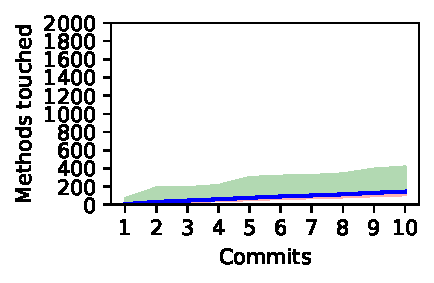
\includegraphics[width=\textwidth]{sections/results/methods/time_series_components_touched.methods.moderate.later.joiner.commits_10.pdf}
    \caption{Moderate later joiner (n=580, $\mu$=145.21, median=38.0 \& std=142.87)}
    \label{subfig:sections/results/methods/time_series_components_touched_methods_moderate_later_joiner_commits_10_pdf}
  \end{subfigure}
\vspace{3mm}
  \begin{subfigure}[b]{0.45\textwidth}
    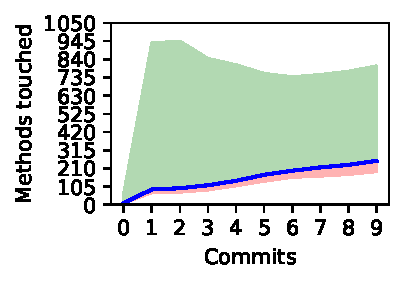
\includegraphics[width=\textwidth]{sections/results/methods/time_series_components_touched.methods.sustained.founder.commits_10.pdf}
    \caption{Sustained founder (n=27, $\mu$=264.52, median=43.0 \& std=380.74)}
    \label{subfig:sections/results/methods/time_series_components_touched_methods_sustained_founder_commits_10_pdf}
  \end{subfigure}
  \begin{subfigure}[b]{0.45\textwidth}
    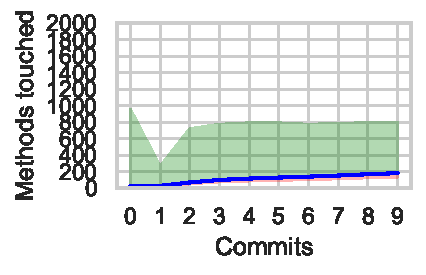
\includegraphics[width=\textwidth]{sections/results/methods/time_series_components_touched.methods.sustained.later.joiner.commits_10.pdf}
    \caption{Sustained later joiner (n=203, $\mu$=180.7, median=34.0 \& std=313.08)}
    \label{subfig:sections/results/methods/time_series_components_touched_methods_sustained_later_joiner_commits_10_pdf}
  \end{subfigure}
\caption[Time Series for methods unit:commits category:4 commits:10]{A time series for the ten (10) commits, excluding transient, with the average mean (blue line), methods touched (y-axis) against the number of commits (x-axis) for four (4) developer categories. Green is the standard deviation above the mean, and pink is the standard deviation below the mean.} 
    \label{fig:codebase_graph_latex_repository_graph_component_time_series_time_series_components_touchedmethods_10_10}
\end{figure}
\clearpage 
